\section{Arduino kode med flere sensore}
For at robotten er i stand til at kunne følge linjen hurtigst og bedst muligt implementeres ydereligere sensore. Dette gøres for at robotten kan navigere nøjagtigt og præcist. Sensorene er placeret ud fra en skabelon som gruppen har 3D printet for at skabe de bedste omstændigheder muligt for at få så præcise måliner som muligt.
\newline 
Her anvendes konceptet vist i figur \ref{line_track} i Line Track. 
\newline


Herfra ændres softwaren fra den indledende problemløsning til at håndtere tre sensore i stedet for én. 

\begin{figure}[h!]
  \centering
  \includegraphics[width=0.5\textwidth]{figures/lineTrackingFlowchartMultibleSensors.png}
  \caption{Software flowchart over problemløsningen ved hjælp af tre sensore i et superloop.}
  \label{flowchart_flere_sensorer}
\end{figure}
\newpage

Som det ses på figur \ref{flowchart_flere_sensorer}, er der fire mulige scenarier som blev præsenteret i figur \ref{line_track}.
Som vist i flowchartet registrerer sensorene om stregen er visuel for sensoren eller ej. Såfremt sensoren registrerer en værdi som fortæller om den er på stregen, kører robotten ligeud indtil en anden værdi måles. 
\newline 
Hvis en anden sensor end den midterste afgiver en måling af den opstillede bane angiver dette at banens forløb har ændret sig, og robotten anvender derved de to funktioner anvist i flowchartet hvorvidt der skal justeres til venstre eller højre. 
\newline
Såfremt ingen fejlmålinger fra sensoren eller snavs stopper robotten fortsætter denne i et superloop.
\newpage

Ved videre implementering af yderligere sensore kan målinger fra den enekelte sensor sammenlignes med gennemsnittet af de andre.

\subsubsection{Videreudvikling af Arduino kode}
\begin{figure}[h!]
  \centering
  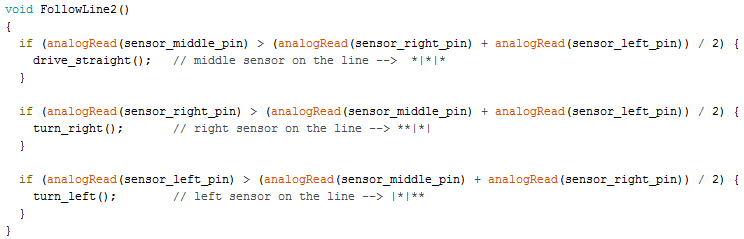
\includegraphics[width=1.0\textwidth]{figures/followLine3.png}
  \caption{Uddrag af den anvendte Arduino kode til problemløsningen med tre sensorer.}
  \label{tre_sensore_followline}
\end{figure}
\newpage

\section{Test og delkonklussion}
Testen er udført på samme bane og med samme fremgangsmåde som testen med anvendelse af én sensor. Robotten foretog adskellige omgange uden at registrere målinger som afsporede robotten. Det kan konkluderes at afstanden imellem sensorene var for stor, hvilket medførte at robotten reagerede sent på målinger fra sensorene i siderne. Dette resulterede i at robotten ikke er i stand til at følge banen hurtigst og bedst muligt. 
PID ville forbedre dette problem. Gruppen har valgt at frapriotere denne mulighed på grund af manglende tid og derfor har valgt at lægge fokus på implementerign af software til embedded. 



\begin{figure}[h!]
  \centering
  \includegraphics[width=0.6\textwidth]{figures/test3sensore.png}
  \caption{Test af Arduino kode med tre anvedte sensore.}
  \label{test_3_sensore}
\end{figure}








%fordel ved flere sensor (behøves ikke reference)
%intro til test
%foklar hvordan testen er udført
%afstand imellem sensor


